\documentclass[11pt]{article}
\usepackage{mathunal-base}
\mathunalfuente{serif}
\providecommand{\nota}[1]{\par\smallskip\noindent{\small\itshape\color{unalblue}#1}\par\smallskip}
\newlist{opciones}{enumerate}{1}
\setlist[opciones]{label=(\alph*),itemsep=1pt,topsep=2pt,leftmargin=1.8em,font=\normalfont}
\newcommand{\rp}{\underline{\hspace{3cm}}}

\renewcommand{\examtitulo}{Ecuaciones Diferenciales (1000007) --- Segundo Examen Parcial}
\renewcommand{\examfecha}{23 de Octubre del 2017}

\begin{document}

\examheader

\vspace{4pt}
\noindent\textit{El examen consta de cinco preguntas en tres hojas impresas por ambos lados. Antes de empezar verifique que su examen esté completo y que sus datos sean correctos. En las preguntas con procedimiento justifique sus respuestas en los espacios asignados. No está permitido hacer preguntas, usar calculadoras, sacar hojas en blanco ni ningún tipo de apuntes durante el examen. Por favor verifique que su celular esté apagado.}

\vspace{6pt}
\noindent\textbf{1. [20pt]} Las raíces de la ecuación $r^2-2r+5=0$ son $r_1=1+2i$ y $r_2=1-2i$. Usando este hecho, halle la solución general de la ecuación diferencial
\[
y''-2y'+5y=e^{x}\tan(2x)
\]
en el intervalo $\left(0,\dfrac{\pi}{4}\right)$.

\nota{Indicación: puede usar la siguiente fórmula $\displaystyle\int \sec t\,dt=\ln|\sec t+\tan t|+C$.}

\vspace{6cm}

\newpage

\noindent\textbf{2. [25pt]}

\vspace{0.2cm}
\noindent\textbf{(a) [10pt]} Una masa que pesa 4 lbs hace que se alargue $\frac{1}{6}$ pies un resorte. Después de estar en equilibrio, la masa se hala hacia abajo $\frac{1}{2}$ pies y se suelta desde el reposo. Sobre el sistema masa-resorte no hay fuerza de amortiguamiento, y una fuerza externa de $5\cos(2t)$ lbs actúa sobre la masa. Formule con precisión el PVI que describe el movimiento de la masa (no es necesario que lo resuelva, ni tal solución será tenida en cuenta).

\vspace{4cm}

\noindent\textbf{(b) [15pt]} La posición $x(t)$ de cierto sistema masa-resorte satisface el problema de valor inicial
\[
\frac{3}{2}x''(t)+kx(t)=0, \qquad x(0)=2,\ x'(0)=\gamma,
\]
donde $k$ y $\gamma$ son constantes positivas. Si el periodo $T$ y la amplitud $R$ del movimiento resultante son $2\pi$ y $4$, respectivamente, determine los valores de $k$ y $\gamma$.

\vspace{6cm}

\newpage

\noindent\textbf{3. [15pt]}

\vspace{0.2cm}
\noindent\textbf{(a) [10pt]} Demuestre que las funciones $y_1$, $y_2$ y $y_3$ cuyas gráficas se presentan en la figura son linealmente independientes en el intervalo $(0.9,\,4.1)$.

\begin{center}
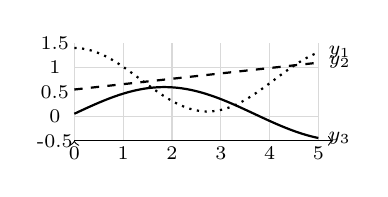
\begin{tikzpicture}[scale=0.62]
\draw[gray!30,thin] (0,-0.5) grid (5,1.5);
\draw[->] (0,-0.5) -- (5.3,-0.5) node[right,font=\scriptsize] {};
\draw[->] (0,-0.5) -- (0,-0.5);
\foreach \x in {0,1,2,3,4,5}{\node[font=\scriptsize] at (\x,-0.75) {\x};}
\foreach \y in {-0.5,0,0.5,1,1.5}{\node[font=\scriptsize] at (-0.4,\y) {\y};}
\draw[thick,domain=0:5,samples=60,dotted] plot(\x,{0.75+0.65*cos(1.15*\x r)}) node[right,font=\scriptsize]{$y_1$};
\draw[thick,domain=0:5,samples=60,dashed] plot(\x,{0.55+0.11*\x}) node[right,font=\scriptsize]{$y_2$};
\draw[thick,domain=0:5,samples=60] plot(\x,{0.05+0.55*sin(0.85*\x r + 0.3)}) node[right,font=\scriptsize]{$y_3$};
\end{tikzpicture}
\end{center}
\nota{Figura esquemática (redibujada): lo relevante son los cruces de las tres curvas en el intervalo, no sus valores exactos. Indicación: analice qué sucede al evaluar la expresión $c_1y_1(x)+c_2y_2(x)+c_3y_3(x)=0$ en $x=2$.}

\vspace{0.3cm}
\noindent\textbf{(b) [5pt]} El Wronskiano de dos funciones $f$ y $g$ es $W(x)=x^3-8$, para cada $x\in(0,3)$. Determine si las funciones $f$ y $g$ son L.I. o L.D. en tal intervalo. Justifique su respuesta.

\vspace{3cm}

\newpage

\noindent\textbf{NOTA:} En las preguntas 4 y 5, se califica sólo la respuesta y no se tiene en cuenta el procedimiento.

\vspace{0.3cm}
\noindent\textbf{4. [20pt]} Escriba claramente su respuesta en la línea correspondiente.

\vspace{0.2cm}
\noindent\textbf{(a) [8pt]} Una forma adecuada de solución particular para la ecuación diferencial
\[
y^{(4)}+4y'''+5y''=4+e^{x}+e^{-2x}\sin x
\]
es \rp\ (no halle las constantes).

\vspace{0.3cm}
\noindent\textbf{(b) [6pt]} El valor de $c$ para que $y=e^{-x}$ sea una solución de la ED homogénea
\[
y'''+cy''+4y'+2y=0
\]
es \rp

\vspace{0.3cm}
\noindent\textbf{(c) [6pt]} Sabiendo que $y=x^2\cos(\ln x)$ y $x^2\sin(\ln x)$ son soluciones de una ED de Cauchy-Euler homogénea de orden 2 en $(0,\infty)$, escriba dicha ecuación diferencial: \rp

\vspace{1cm}

\noindent\textbf{5. [20pt]} En este problema denotamos a una ecuación diferencial lineal homogénea de orden $n$, con coeficientes constantes como
\[
a_n\frac{d^ny}{dx^n}+\cdots+a_1\frac{dy}{dx}+a_0y=0, \tag{1}
\]
donde $a_i\in\mathbb{R}$ para todo $i=0,1,\ldots,n$, y $a_n\neq 0$. Recuerde que para la Ecuación (1), la ecuación característica asociada viene dada por
\[
a_nr^n+\cdots+a_1r+a_0=0. \tag{2}
\]
Los siguientes literales se refieren a las funciones $z_1,\ldots,z_4$ definidas en $\mathbb{R}$ cuyas porciones de gráficas se indican a continuación.

\begin{center}
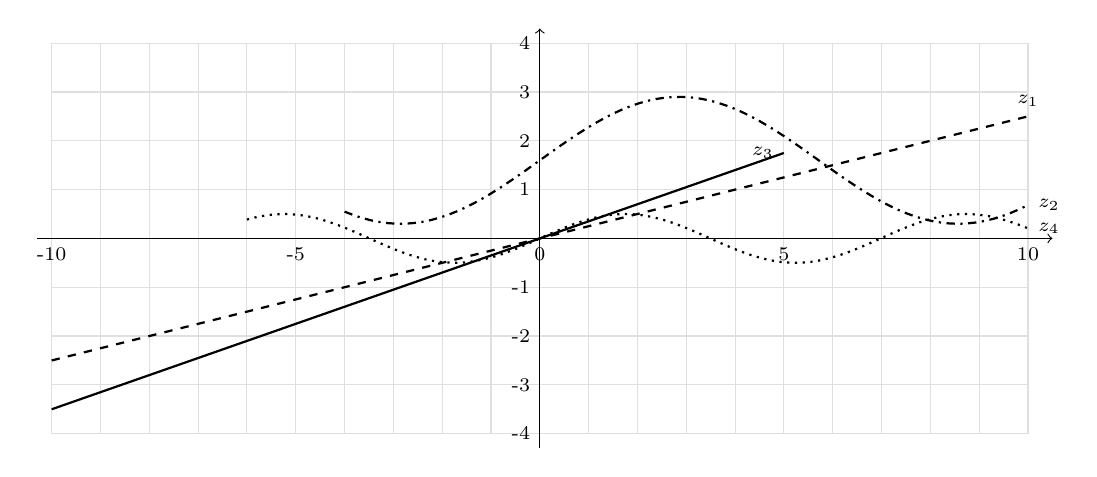
\begin{tikzpicture}[scale=0.62]
\draw[gray!25,thin] (-10,-4) grid (10,4);
\draw[->] (-10.3,0) -- (10.5,0);
\draw[->] (0,-4.3) -- (0,4.3);
\foreach \x in {-10,-5,0,5,10}{\node[below,font=\scriptsize] at (\x,0) {\x};}
\foreach \y in {-4,-3,-2,-1,1,2,3,4}{\node[left,font=\scriptsize] at (0,\y) {\y};}
\draw[thick,domain=-10:10,samples=80,dashed] plot(\x,{\x/4}) node[above,font=\scriptsize]{$z_1$};
\draw[thick,domain=-4:10,samples=80,dash dot] plot(\x,{1.6+1.3*sin(0.55*\x r)}) node[right,font=\scriptsize]{$z_2$};
\draw[thick,domain=-10:5,samples=80] plot(\x,{0.35*\x}) node[left,font=\scriptsize]{$z_3$};
\draw[thick,domain=-6:10,samples=80,dotted] plot(\x,{0.5*sin(0.9*\x r)}) node[right,font=\scriptsize]{$z_4$};
\end{tikzpicture}
\end{center}
\nota{Figura esquemática (redibujada): representa el tipo de comportamiento (creciente/decreciente, oscilatorio, acotado) de cada función, no sus valores exactos.}

\begin{opciones}
\item[(a)] \textbf{[5pt]} Si $z_1\cdot z_3$ es una solución de la ED (1) en $\mathbb{R}$ y $z_i\cdot z_j$ es una solución de (1) en $\mathbb{R}$ linealmente independiente de $z_1\cdot z_3$ entonces $i=$~\underline{\hspace{1.2cm}}, $j=$~\underline{\hspace{1.2cm}}.
\item[(b)] \textbf{[5pt]} Si la ecuación (2) es $r^2+c^2=0$ con $c\in\mathbb{R}$, y la solución de la Ecuación (1) en $\mathbb{R}$ tiene la estructura $y=c_1z_i+c_2z_j$ entonces $i=$~\underline{\hspace{1.2cm}}, $j=$~\underline{\hspace{1.2cm}}.
\item[(c)] \textbf{[5pt]} Si la Ecuación (2) se escribe $(r-a)(r-b)=0$ con $a<0<b$ números reales, y la solución de la Ecuación (1) en $\mathbb{R}$ tiene la estructura $y=c_1z_i+c_2z_j$ entonces $i=$~\underline{\hspace{1.2cm}}, $j=$~\underline{\hspace{1.2cm}}.
\item[(d)] \textbf{[5pt]} Si la Ecuación (2) tiene una única raíz real positiva y $z_i$ es solución de (1) en $\mathbb{R}$, entonces $i=$~\underline{\hspace{1.2cm}}.
\end{opciones}

\vfill
\rule{\linewidth}{0.4pt}\\[1pt]
{\scriptsize\textit{Transcripción digital --- MathUNAL}\hfill\textcolor{unalblue}{\textbf{1}}}

\end{document}
